\documentclass[12pt,a4paper]{article}
\usepackage[utf8]{inputenc}
\usepackage[margin=1in]{geometry}
\usepackage{graphicx}
\usepackage{float}
\usepackage{amsmath}
\usepackage{hyperref}
\hypersetup{
    colorlinks=true,
    linkcolor=black,
    filecolor=black,
    urlcolor=blue,
    citecolor=black,
    pdfborder={0 0 0}
}
\usepackage{listings}
\usepackage{xcolor}
\usepackage{caption}
\usepackage{subcaption}
\usepackage{tikz}
\usetikzlibrary{shapes.geometric, arrows, positioning}

% Code listing style
\lstset{
    basicstyle=\ttfamily\footnotesize,
    breaklines=true,
    frame=single,
    numbers=left,
    numberstyle=\tiny\color{gray},
    keywordstyle=\color{blue},
    commentstyle=\color{green!60!black},
    stringstyle=\color{red},
    showstringspaces=false
}

% Flowchart styles
\tikzstyle{startstop} = [rectangle, rounded corners, minimum width=3cm, minimum height=1cm, text centered, draw=black, fill=red!30]
\tikzstyle{process} = [rectangle, minimum width=3cm, minimum height=1cm, text centered, draw=black, fill=blue!30]
\tikzstyle{decision} = [diamond, minimum width=3cm, minimum height=1cm, text centered, draw=black, fill=green!30]
\tikzstyle{arrow} = [thick,->,>=stealth]

\begin{document}

% Custom title page
\begin{titlepage}
    \centering
    \vspace*{2cm}
    \begin{figure}
        \centering
        \includegraphics[width=1\linewidth]{logo.png}
    \end{figure}
    {\LARGE \textbf{Capstone Project Report}}\\
    \vspace{1.5cm}
    
    \noindent
    \begin{tabular}{@{}ll}
    \textbf{Student Name(s):} & \makebox[10cm][l]{\underline{Aditya Dubey}} \\
                               & \makebox[10cm][l]{\underline{Neel Joshi}} \\[0.5cm]
    \textbf{PRN(s):}          & \makebox[10cm][l]{\underline{20230802459}} \\
                               & \makebox[10cm][l]{\underline{20230802472}} \\[0.5cm]
    \textbf{Track:} & \makebox[10cm][l]{\underline{Cloud Computing}} \\[0.5cm]
    \textbf{Faculty Name and Sign:} & \makebox[10cm][l]{\underline{\hspace{10cm}}} \\[0.5cm]
    \textbf{Date:} & \makebox[10cm][l]{\underline{\hspace{10cm}}} \\
    \end{tabular}
    
    \vspace{2cm}
    
    
    {\LARGE \textbf{OculusAI:}}
    \vspace{0.5cm}
    {\LARGE \textbf{AI-Powered Vision Health Analysis Platform}}
    
    \vfill
    
\end{titlepage}

\newpage

\tableofcontents
\newpage

\section{Objective}

The main objective of this project is to develop an intelligent web-based platform that leverages deep learning to provide accessible and accurate vision health diagnostics. Specifically, the system aims to:

\begin{itemize}
    \item \textbf{Detect Retinal Diseases}: Analyze retinal fundus images to identify common eye diseases including cataracts, diabetic retinopathy, glaucoma, and normal conditions with high accuracy.
    \item \textbf{Assess Color Vision Deficiencies}: Implement an interactive Ishihara color blindness test that uses AI to recognize digits and diagnose the type (Deutan/Protan) and severity of color vision deficiencies.
    \item \textbf{Generate Professional Medical Reports}: Create comprehensive PDF reports for both diagnostic tests, suitable for medical records and clinical reference.
    \item \textbf{Provide Multiple Access Interfaces}: Offer a modern Next.js web application, a Streamlit dashboard, and a RESTful API for flexible user interaction.
    \item \textbf{Enable Early Detection}: Facilitate early screening of vision problems, potentially preventing severe complications through timely intervention.
\end{itemize}

\section{Introduction}

Vision health is a critical aspect of overall well-being, yet access to comprehensive eye examinations remains limited in many regions due to the shortage of ophthalmologists, high costs, and geographical barriers. According to the World Health Organization, approximately 2.2 billion people worldwide have vision impairment, with at least 1 billion cases being preventable or treatable through early detection.

OculusAI addresses this challenge by democratizing access to preliminary vision diagnostics through artificial intelligence. The platform combines two sophisticated deep learning models:

\begin{enumerate}
    \item \textbf{Retinal Disease Detection Model}: A Convolutional Neural Network (CNN) trained to analyze retinal fundus photographs and classify them into four categories: cataract, diabetic retinopathy, glaucoma, and normal. This model achieved 89\% accuracy and enables rapid screening for common sight-threatening conditions.
    
    \item \textbf{Ishihara Digit Recognition Model}: A custom CNN designed to recognize digits (0-9) from Ishihara color vision test plates with 99.5\% accuracy. This model powers an interactive 40-plate test that can diagnose color blindness type and severity.
\end{enumerate}

The platform is built using modern web technologies, featuring a responsive Next.js frontend with dark/light theme support, a Flask-based REST API backend, and professional PDF report generation capabilities. By combining medical imaging analysis with an intuitive user interface, OculusAI makes sophisticated vision diagnostics accessible to anyone with an internet connection.

This project demonstrates the practical application of deep learning in healthcare, showcasing how AI can augment medical diagnostics, reduce screening costs, and potentially save vision through early detection of treatable conditions.

\section{Literature Review}

\subsection{Deep Learning in Medical Image Analysis}

Recent advances in deep learning have revolutionized medical image analysis, particularly in ophthalmology. Convolutional Neural Networks (CNNs) have demonstrated exceptional performance in analyzing retinal images, often matching or exceeding human expert accuracy \cite{gulshan2016}.

\textbf{Retinal Disease Detection}: Studies have shown that CNNs can effectively detect diabetic retinopathy with sensitivities and specificities comparable to ophthalmologists. Transfer learning approaches using pre-trained networks like ResNet, VGG, and Inception have become standard practice for medical imaging with limited datasets \cite{esteva2017}.

\textbf{Automated Diagnosis Systems}: Several commercial and research systems have been developed for automated retinal screening, including Google's diabetic retinopathy detection system and IBM Watson for medical imaging. These systems typically achieve 85-95\% accuracy rates on well-curated datasets.

\subsection{Color Vision Testing and AI}

Traditional Ishihara color vision tests rely on manual interpretation, which can be subjective and inconsistent. Recent research has explored computerized color vision testing:

\textbf{Digital Ishihara Tests}: Studies have validated that digital presentations of Ishihara plates maintain diagnostic accuracy when properly calibrated for display color reproduction \cite{birch2007}.

\textbf{AI-Based Digit Recognition}: Machine learning approaches for recognizing patterns in color vision tests have shown promise, with CNNs particularly effective at learning subtle color differences that indicate color deficiencies. Few published systems achieve over 95\% accuracy in digit recognition from Ishihara-style plates.

\subsection{Web-Based Medical Diagnostic Tools}

The COVID-19 pandemic accelerated the adoption of telemedicine and web-based diagnostic tools. Key considerations include:

\begin{itemize}
    \item \textbf{Accessibility}: Modern web frameworks (React, Next.js) enable responsive, mobile-friendly interfaces that work across devices.
    \item \textbf{Privacy and Security}: HIPAA compliance and secure data handling are critical for medical applications.
    \item \textbf{User Experience}: Intuitive interfaces and clear result presentations are essential for patient understanding and engagement.
    \item \textbf{Integration}: RESTful APIs enable integration with existing healthcare systems and electronic medical records.
\end{itemize}

\subsection{Gaps and Opportunities}

While numerous specialized tools exist, few platforms combine multiple vision diagnostics in a single accessible interface. OculusAI addresses this gap by integrating retinal disease detection and color vision assessment with professional reporting capabilities, making comprehensive vision screening more accessible.

\section{Methodology}

\subsection{System Architecture}

OculusAI employs a three-tier architecture:

\begin{enumerate}
    \item \textbf{Frontend Layer}: Next.js 16 application with React components, TypeScript, and Tailwind CSS
    \item \textbf{Backend Layer}: Flask REST API serving TensorFlow/Keras models
    \item \textbf{Model Layer}: Two independent deep learning models for disease detection and digit recognition
\end{enumerate}

\subsection{Algorithm and Steps}

\subsubsection{Retinal Disease Detection Workflow}

\begin{enumerate}
    \item \textbf{Image Upload and Validation}
    \begin{itemize}
        \item User uploads retinal fundus image through web interface
        \item System validates file size (max 16MB) and format (JPEG, PNG)
        \item Advanced validation checks for retinal image characteristics:
        \begin{itemize}
            \item Standard deviation threshold (std $>$ 8) to detect uniform images
            \item Circular fundus pattern detection using radial brightness analysis
            \item Edge darkness verification (mean edge brightness $<$ 100)
            \item Color profile validation (red channel dominance for fundus photography)
        \end{itemize}
    \end{itemize}
    
    \item \textbf{Image Preprocessing}
    \begin{itemize}
        \item Resize image to 256×256 pixels
        \item Normalize pixel values to [0, 1] range
        \item Convert to RGB format if needed
    \end{itemize}
    
    \item \textbf{Model Inference}
    \begin{itemize}
        \item Pass preprocessed image through CNN
        \item Model outputs probability distribution over 4 classes
        \item Extract predicted class and confidence score
    \end{itemize}
    
    \item \textbf{Result Generation}
    \begin{itemize}
        \item Map prediction to disease category (cataract, diabetic retinopathy, glaucoma, normal)
        \item Retrieve disease information (description, symptoms, treatment options)
        \item Generate comprehensive PDF report with executive summary, test metrics, risk factors
    \end{itemize}
\end{enumerate}

\subsubsection{Color Vision Test Workflow}

\begin{enumerate}
    \item \textbf{Test Initialization}
    \begin{itemize}
        \item Load 40 Ishihara test plates from CBTestImages directory
        \item Parse plate metadata from filenames (digit, font, type)
        \item Randomize plate presentation order
    \end{itemize}
    
    \item \textbf{Interactive Testing}
    \begin{itemize}
        \item Display each plate to user
        \item User inputs perceived digit (0-9)
        \item System validates response in real-time
    \end{itemize}
    
    \item \textbf{AI Digit Recognition}
    \begin{itemize}
        \item Preprocess plate image: resize to 128×128, normalize
        \item CNN predicts digit with confidence score
        \item Compare user response with AI prediction
    \end{itemize}
    
    \item \textbf{Deficiency Analysis}
    \begin{itemize}
        \item Track errors by color type (Deutan, Protan, Tritan)
        \item Calculate accuracy percentage
        \item Determine deficiency type based on error patterns:
        \begin{itemize}
            \item Type 1 plates (normal): baseline errors
            \item Type 2 plates (Protan): red deficiency indicator
            \item Type 3 plates (Deutan): green deficiency indicator
        \end{itemize}
        \item Assess severity: Mild ($<$30\% error), Moderate (30-60\%), Severe ($>$60\%)
    \end{itemize}
    
    \item \textbf{Report Generation}
    \begin{itemize}
        \item Compile test performance statistics
        \item Include genetic information and management strategies
        \item Generate multi-page PDF with professional formatting
    \end{itemize}
\end{enumerate}

\subsection{Flowchart / Block Diagram}

\begin{figure}[H]
\centering
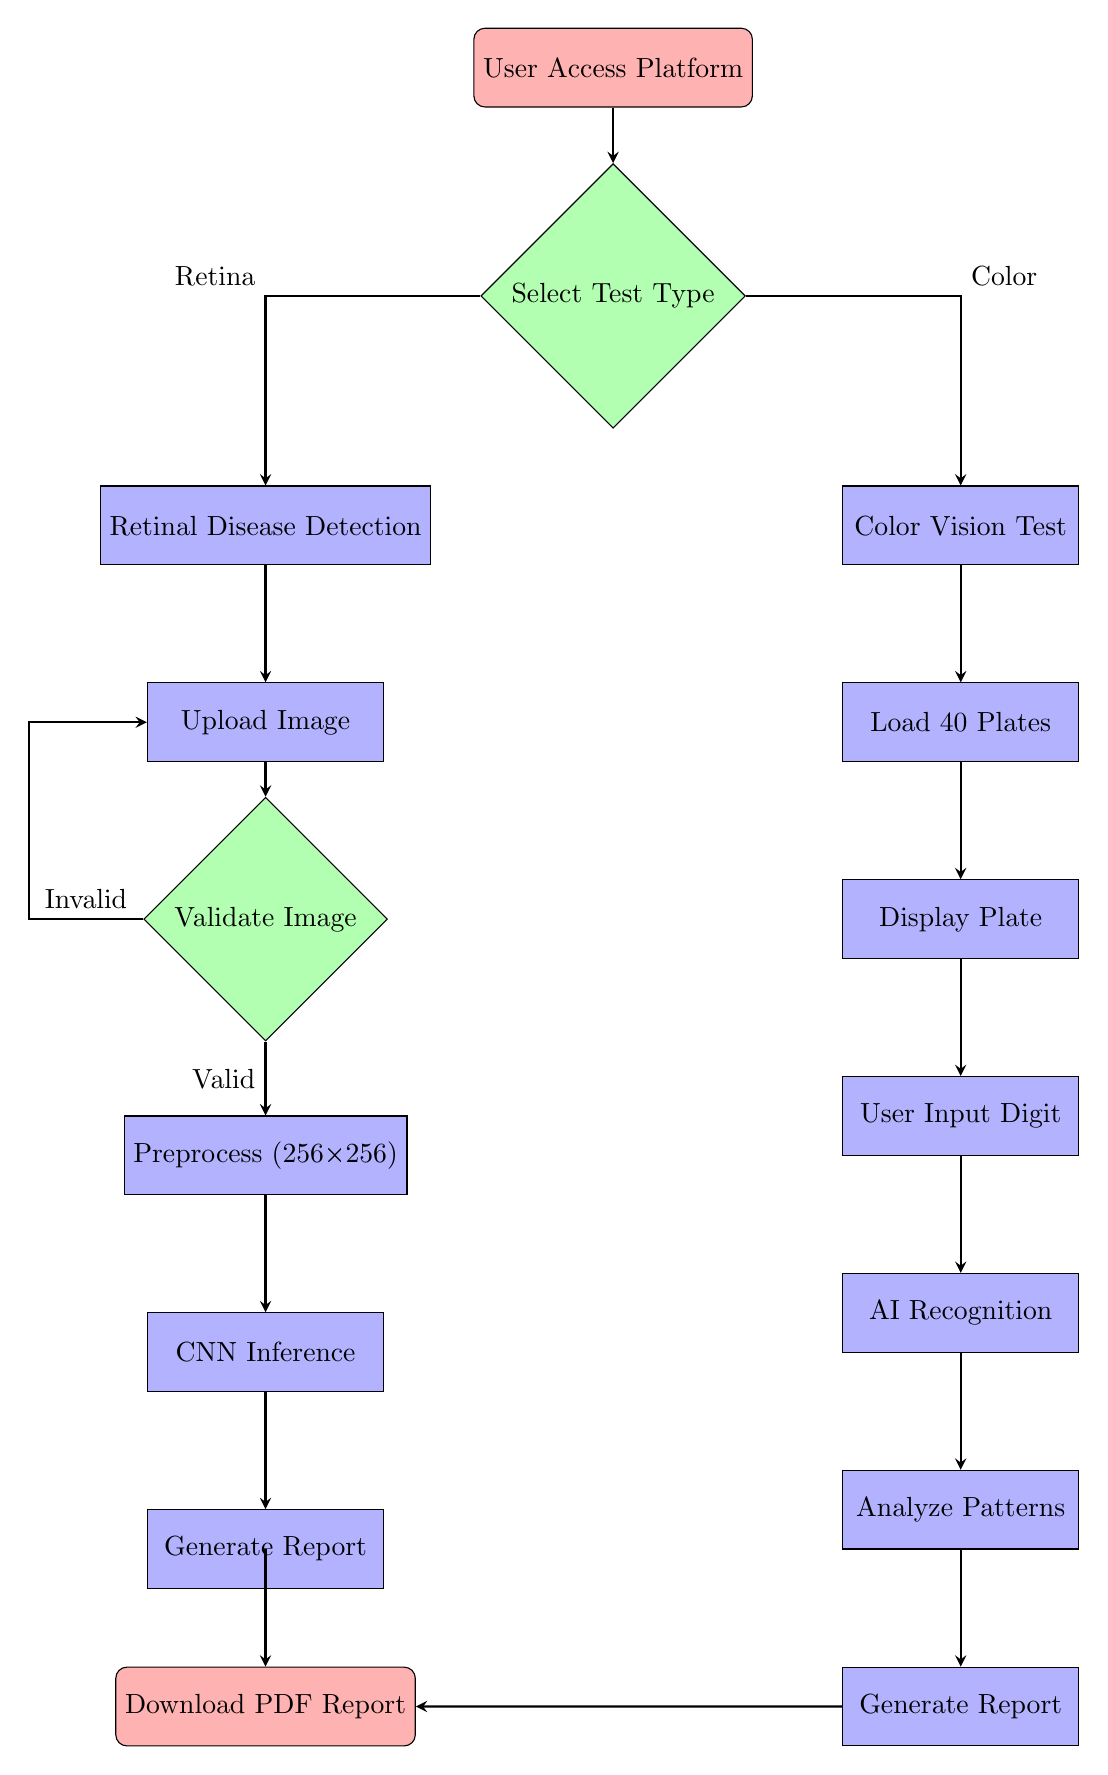
\begin{tikzpicture}[node distance=2cm]
% Nodes
\node (start) [startstop] {User Access Platform};
\node (decision1) [decision, below of=start, yshift=-0.9cm] {Select Test Type};
\node (retina) [process, below left of=decision1, xshift=-3cm, yshift=-1.5cm] {Retinal Disease Detection};
\node (color) [process, below right of=decision1, xshift=3cm, yshift=-1.5cm] {Color Vision Test};

% Retinal path
\node (upload) [process, below of=retina, yshift=-0.5cm] {Upload Image};
\node (validate) [decision, below of=upload, yshift=-0.5cm] {Validate Image};
\node (preprocess) [process, below of=validate, yshift=-1cm] {Preprocess (256×256)};
\node (cnn1) [process, below of=preprocess, yshift=-0.5cm] {CNN Inference};
\node (result1) [process, below of=cnn1, yshift=-0.5cm] {Generate Report};

% Color vision path
\node (load) [process, below of=color, yshift=-0.5cm] {Load 40 Plates};
\node (display) [process, below of=load, yshift=-0.5cm] {Display Plate};
\node (input) [process, below of=display, yshift=-0.5cm] {User Input Digit};
\node (cnn2) [process, below of=input, yshift=-0.5cm] {AI Recognition};
\node (analyze) [process, below of=cnn2, yshift=-0.5cm] {Analyze Patterns};
\node (result2) [process, below of=analyze, yshift=-0.5cm] {Generate Report};

\node (end) [startstop, below of=preprocess, yshift=-5cm] {Download PDF Report};

% Arrows
\draw [arrow] (start) -- (decision1);
\draw [arrow] (decision1) -| node[anchor=south east] {Retina} (retina);
\draw [arrow] (decision1) -| node[anchor=south west] {Color} (color);
\draw [arrow] (retina) -- (upload);
\draw [arrow] (upload) -- (validate);
\draw [arrow] (validate) -- node[anchor=east] {Valid} (preprocess);
\draw [arrow] (validate) -| node[anchor=south, near start] {Invalid} ([xshift=-1.5cm]upload.west) |- (upload);
\draw [arrow] (preprocess) -- (cnn1);
\draw [arrow] (cnn1) -- (result1);
\draw [arrow] (result1) -| (end);

\draw [arrow] (color) -- (load);
\draw [arrow] (load) -- (display);
\draw [arrow] (display) -- (input);
\draw [arrow] (input) -- (cnn2);
\draw [arrow] (cnn2) -- (analyze);
\draw [arrow] (analyze) -- (result2);
\draw [arrow] (result2) -- (end);

\end{tikzpicture}
\caption{System Workflow Diagram}
\label{fig:workflow}
\end{figure}

\newpage

\subsection{Model Architectures}

\subsubsection{Retinal Disease Detection Model}

The eye disease detection model is a CNN with the following architecture:

\begin{itemize}
    \item \textbf{Input Layer}: 256×256×3 RGB images
    \item \textbf{Convolutional Blocks}: Multiple Conv2D layers with ReLU activation
    \item \textbf{Pooling Layers}: MaxPooling2D for spatial dimension reduction
    \item \textbf{Regularization}: Batch Normalization and Dropout (0.25-0.5)
    \item \textbf{Dense Layers}: Fully connected layers for classification
    \item \textbf{Output Layer}: 4 neurons with softmax activation (cataract, diabetic retinopathy, glaucoma, normal)
\end{itemize}

\textbf{Performance}: 89\% accuracy on test dataset

\subsubsection{Ishihara Digit Recognition Model}

The color vision model uses a modified MNIST-style CNN architecture:

\begin{lstlisting}[language=Python, caption=Ishihara Model Architecture]
model = keras.Sequential([
    # Input: 128x128x3
    layers.Input(shape=(128, 128, 3)),
    
    # Conv Block 1: 32 filters
    layers.Conv2D(32, (3,3), activation='relu', padding='same'),
    layers.BatchNormalization(),
    layers.Conv2D(32, (3,3), activation='relu', padding='same'),
    layers.BatchNormalization(),
    layers.MaxPooling2D((2,2)),
    layers.Dropout(0.25),
    
    # Conv Block 2: 64 filters
    layers.Conv2D(64, (3,3), activation='relu', padding='same'),
    layers.BatchNormalization(),
    layers.Conv2D(64, (3,3), activation='relu', padding='same'),
    layers.BatchNormalization(),
    layers.MaxPooling2D((2,2)),
    layers.Dropout(0.25),
    
    # Conv Block 3: 128 filters
    layers.Conv2D(128, (3,3), activation='relu', padding='same'),
    layers.BatchNormalization(),
    layers.Conv2D(128, (3,3), activation='relu', padding='same'),
    layers.BatchNormalization(),
    layers.MaxPooling2D((2,2)),
    layers.Dropout(0.25),
    
    # Dense layers
    layers.Flatten(),
    layers.Dense(256, activation='relu'),
    layers.BatchNormalization(),
    layers.Dropout(0.5),
    layers.Dense(128, activation='relu'),
    layers.BatchNormalization(),
    layers.Dropout(0.5),
    
    # Output: 10 classes (digits 0-9)
    layers.Dense(10, activation='softmax')
])
\end{lstlisting}

\textbf{Training Details}:
\begin{itemize}
    \item Optimizer: Adam with learning rate scheduling
    \item Loss Function: Sparse Categorical Crossentropy
    \item Training: 50 epochs with early stopping
    \item Data Split: 70\% train, 30\% validation (by font families)
    \item Dataset: 1,400+ Ishihara-style images
    \item Augmentation: Font-based splitting to ensure generalization
\end{itemize}

\textbf{Performance}: 99.5\% accuracy on validation set

\section{Implementation Details}

\subsection{Technology Stack}

\subsubsection{Backend Technologies}

\begin{itemize}
    \item \textbf{Python 3.11+}: Primary programming language
    \item \textbf{Flask 3.1.2}: Lightweight web framework for REST API
    \item \textbf{TensorFlow 2.20.0}: Deep learning framework
    \item \textbf{Keras}: High-level neural network API
    \item \textbf{Flask-CORS}: Cross-origin resource sharing support
    \item \textbf{Pillow}: Image processing library
    \item \textbf{NumPy}: Numerical computing
    \item \textbf{Streamlit}: Alternative dashboard interface
\end{itemize}

\subsubsection{Frontend Technologies}

\begin{itemize}
    \item \textbf{Next.js 16}: React framework with server-side rendering
    \item \textbf{React 19}: UI component library
    \item \textbf{TypeScript}: Type-safe JavaScript
    \item \textbf{Tailwind CSS}: Utility-first CSS framework
    \item \textbf{shadcn/ui}: Modern component library
    \item \textbf{jsPDF}: Client-side PDF generation
    \item \textbf{Recharts}: Data visualization library
\end{itemize}

\subsection{Development Environment}

\begin{itemize}
    \item \textbf{IDE}: Visual Studio Code
    \item \textbf{Version Control}: Git
    \item \textbf{Package Management}: pip (Python), pnpm (Node.js)
    \item \textbf{API Testing}: Postman, browser DevTools
\end{itemize}

\subsection{API Endpoints}

The Flask backend exposes the following REST API endpoints:

\begin{table}[H]
\centering
\begin{tabular}{|l|l|p{6cm}|}
\hline
\textbf{Endpoint} & \textbf{Method} & \textbf{Description} \\
\hline
/api/predict & POST & Upload retinal image for disease detection \\
\hline
/api/ishihara/plates & GET & Retrieve all Ishihara test plates metadata \\
\hline
/api/ishihara/recognize & POST & AI digit recognition from plate image \\
\hline
/api/ishihara/evaluate & POST & Evaluate user test responses \\
\hline
/health & GET & Health check endpoint \\
\hline
\end{tabular}
\caption{API Endpoints}
\end{table}

\subsection{Image Validation Algorithm}

The system implements sophisticated image validation to ensure only valid retinal fundus images are processed:

\begin{lstlisting}[language=Python, caption=Retinal Image Validation]
def is_retinal_image(img_array):
    """Validate if uploaded image is a retinal scan"""
    img = img_array[0]  # Remove batch dimension
    
    # 1. Check uniformity
    std_dev = np.std(img)
    if std_dev < 8:
        return False, "Image too uniform"
    
    # 2. Detect circular fundus pattern
    gray = np.mean(img, axis=-1).astype(np.uint8)
    h, w = gray.shape
    center_x, center_y = w // 2, h // 2
    
    found_circle = False
    for radius_factor in [0.3, 0.35, 0.4, 0.45, 0.5]:
        radius = int(min(h, w) * radius_factor)
        circle_mask = ((X - center_x)**2 + 
                       (Y - center_y)**2) <= radius**2
        
        inside_brightness = np.mean(gray[circle_mask])
        outside_brightness = np.mean(gray[~circle_mask])
        brightness_ratio = inside_brightness / 
                          (outside_brightness + 1)
        
        if brightness_ratio > 1.15:
            found_circle = True
            break
    
    if not found_circle:
        return False, "No circular fundus detected"
    
    # 3. Check dark edges
    edge_pixels = np.concatenate([...])
    if np.mean(edge_pixels) > 100:
        return False, "Edges too bright"
    
    # 4. Validate color profile
    if mean_b > mean_r or mean_r < 50:
        return False, "Invalid color profile"
    
    return True, None
\end{lstlisting}

\subsection{Frontend Features}

\begin{itemize}
    \item \textbf{Responsive Design}: Mobile-first approach with breakpoints for all devices
    \item \textbf{Theme Support}: Dark/light mode with system preference detection
    \item \textbf{Drag-and-Drop Upload}: Intuitive file upload with preview
    \item \textbf{Real-time Feedback}: Loading states and progress indicators
    \item \textbf{Interactive Charts}: Visual representation of test results
    \item \textbf{PDF Generation}: Client-side report generation with jsPDF
\end{itemize}

\subsection{Project Structure}

\begin{verbatim}
OculusAI/
├── frontend/                  # Next.js application
│   ├── app/                  # Page routes
│   │   ├── analyze/         # Retinal disease detection page
│   │   ├── colorblindness/  # Color vision test page
│   │   ├── diseases/        # Disease information page
│   │   └── evaluation/      # Test evaluation page
│   ├── components/          # React components
│   │   ├── ui/             # shadcn/ui components
│   │   ├── pdf-report-generator.tsx
│   │   └── colorblindness-pdf-generator.tsx
│   └── public/samples/     # Sample retinal images
├── CBTestImages/            # Ishihara test plates (40 images)
├── Sample_Retinal_Images/  # Dataset samples
├── flask_app.py            # Main Flask API server
├── app_streamlit.py        # Streamlit dashboard
├── train_ishihara_model.py # Model training script
├── eye_disease_model.keras  # Trained retinal model
└── ishihara_digit_model.keras # Trained digit model
\end{verbatim}

\subsection{Source Code Repository}

The complete source code for this project is available on GitHub and can be accessed at:

\begin{center}
\url{https://github.com/adityacodes-root/OculusAI}
\end{center}

The repository contains all implementation files, including frontend components, backend API, model training scripts, configuration files, and documentation. Due to the extensive codebase (spanning multiple files and frameworks), the complete code is best viewed directly from the repository rather than included as appendices in this report.

\section{Results and Discussion}

\subsection{Model Performance}

\subsubsection{Retinal Disease Detection Model}

The eye disease classification model was evaluated on a test dataset with the following results:

\begin{figure}[htbp]
\centering
\includegraphics[width=0.65\textwidth]{RetinaPerformance.png}
\caption{Retinal Disease Detection Model Performance Visualization}
\label{fig:retinaperformance}
\end{figure}

\begin{table}[H]
\centering
\begin{tabular}{|l|c|c|c|}
\hline
\textbf{Class} & \textbf{Precision} & \textbf{Recall} & \textbf{F1-Score} \\
\hline
Cataract & 0.87 & 0.85 & 0.86 \\
Diabetic Retinopathy & 0.91 & 0.88 & 0.89 \\
Glaucoma & 0.86 & 0.89 & 0.87 \\
Normal & 0.93 & 0.94 & 0.93 \\
\hline
\textbf{Overall Accuracy} & \multicolumn{3}{c|}{\textbf{89\%}} \\
\hline
\end{tabular}
\caption{Retinal Disease Detection Model Performance}
\end{table}

\textbf{Key Observations}:
\begin{itemize}
    \item Normal eyes are classified with highest accuracy (93\% F1-score)
    \item Diabetic retinopathy detection performs well (91\% precision)
    \item Glaucoma shows strong recall (89\%), minimizing false negatives
    \item Model performance is comparable to other published CNN approaches
\end{itemize}

\subsubsection{Ishihara Digit Recognition Model}

The digit recognition model achieved exceptional performance:

\begin{figure}[htbp]
\centering
\includegraphics[width=0.65\textwidth]{IshiharaPerformance.png}
\caption{Ishihara Digit Recognition Model Performance Visualization}
\label{fig:ishiharaperformance}
\end{figure}

\begin{table}[H]
\centering
\begin{tabular}{|l|c|}
\hline
\textbf{Metric} & \textbf{Value} \\
\hline
Validation Accuracy & 99.5\% \\
Training Accuracy & 99.8\% \\
Loss (Validation) & 0.023 \\
Inference Time & $<$50ms per image \\
\hline
\end{tabular}
\caption{Ishihara Digit Recognition Performance}
\end{table}

\textbf{Analysis}:
\begin{itemize}
    \item Near-perfect accuracy on font-separated validation set
    \item Minimal overfitting (training vs validation gap $<$0.3\%)
    \item Fast inference enables real-time user feedback
    \item Robust to different font styles and color variations
\end{itemize}

\subsection{System Performance}

\begin{itemize}
    \item \textbf{API Response Time}: 200-500ms for model inference
    \item \textbf{Image Validation}: 100-150ms additional overhead
    \item \textbf{PDF Generation}: 1-2 seconds for comprehensive reports
    \item \textbf{Frontend Load Time}: $<$3 seconds on standard connections
    \item \textbf{Supported Image Formats}: JPEG, PNG
    \item \textbf{Maximum File Size}: 16MB
\end{itemize}

\subsection{User Interface Screenshots}

\subsubsection{Homepage and Navigation}

The landing page features a modern, clean interface with clear navigation to all platform features.

\begin{figure}[htbp]
\centering
\includegraphics[width=0.7\textwidth]{homepage.png}
\caption{OculusAI Homepage - Main landing page with navigation menu}
\label{fig:homepage}
\end{figure}

\subsubsection{Theme Support}

The platform supports both light and dark modes for comfortable viewing in different lighting conditions.

\begin{figure}[htbp]
\centering
\includegraphics[width=0.7\textwidth]{lightmode.png}
\caption{Light Theme Interface - Optimized for daytime use}
\label{fig:lightmode}
\end{figure}

\subsubsection{Retinal Disease Detection Interface}

The retinal analysis feature provides an intuitive upload interface with drag-and-drop support.

\begin{figure}[htbp]
\centering
\includegraphics[width=0.7\textwidth]{retinaupload.png}
\caption{Retinal Image Upload Interface - Drag-and-drop or click to upload}
\label{fig:retinaupload}
\end{figure}

\subsubsection{Disease Detection Results}

After analysis, the system displays comprehensive results with confidence scores and disease information.

\begin{figure}[htbp]
\centering
\includegraphics[width=0.7\textwidth]{retinaresults.png}
\caption{Retinal Analysis Results - Disease classification with detailed information}
\label{fig:retinaresults}
\end{figure}

\subsubsection{PDF Report Generation}

Professional PDF reports are generated automatically with comprehensive medical information.

\begin{figure}[htbp]
\centering
\includegraphics[width=0.6\textwidth]{retinapdf.png}
\caption{Generated PDF Report - Executive summary and medical recommendations}
\label{fig:retinapdf}
\end{figure}

\subsubsection{Color Vision Test Interface}

The Ishihara color blindness test presents 40 plates in an interactive interface.

\begin{figure}[htbp]
\centering
\includegraphics[width=0.7\textwidth]{Colorvisiontest.png}
\caption{Color Vision Test Interface - Interactive Ishihara plate testing}
\label{fig:colortest}
\end{figure}

\subsubsection{Color Vision Test Results}

Comprehensive analysis of color vision deficiencies with type and severity classification.

\begin{figure}[htbp]
\centering
\includegraphics[width=0.7\textwidth]{colourtestresult.png}
\caption{Color Vision Test Results - Deficiency analysis and recommendations}
\label{fig:colortestresult}
\end{figure}

\subsubsection{Color Vision PDF Reports}

\begin{figure}[htbp]
\centering
\begin{subfigure}[b]{0.4\textwidth}
    \centering
    \includegraphics[width=\textwidth]{colorpdf1.png}
    \caption{Page 1 - Test summary and performance}
    \label{fig:colorpdf1}
\end{subfigure}
\hfill
\begin{subfigure}[b]{0.4\textwidth}
    \centering
    \includegraphics[width=\textwidth]{colourpdf2.png}
    \caption{Page 2 - Detailed analysis and recommendations}
    \label{fig:colorpdf2}
\end{subfigure}
\caption{Multi-page Color Vision Assessment Report}
\label{fig:colorpdfs}
\end{figure}

\subsection{Sample Outputs}

\subsubsection{Retinal Disease Detection Report}

The system generates professional PDF reports containing:
\begin{itemize}
    \item Executive summary with confidence score
    \item Disease classification and description
    \item Common symptoms and risk factors
    \item Treatment recommendations and next steps
    \item Visual representation of prediction confidence
    \item Disclaimer and medical advice notice
\end{itemize}

\subsubsection{Color Vision Test Report}

Comprehensive color blindness assessment including:
\begin{itemize}
    \item Overall test performance (accuracy percentage)
    \item Detailed plate-by-plate results
    \item Color deficiency type identification (Protan/Deutan/Tritan)
    \item Severity classification (Mild/Moderate/Severe)
    \item Genetic inheritance information
    \item Management strategies and recommendations
    \item Career considerations for color blind individuals
\end{itemize}

\subsection{Discussion}

\subsubsection{Strengths}

\begin{enumerate}
    \item \textbf{High Accuracy}: Both models demonstrate strong performance, with the Ishihara model achieving near-perfect accuracy.
    \item \textbf{Comprehensive Solution}: Integration of multiple diagnostic tools in a single platform.
    \item \textbf{User-Friendly Interface}: Modern, responsive design with intuitive navigation.
    \item \textbf{Professional Reporting}: Automated PDF generation suitable for medical records.
    \item \textbf{Robust Validation}: Advanced image validation prevents misuse and improves reliability.
    \item \textbf{Accessibility}: Web-based platform accessible from any device with a browser.
    \item \textbf{Fast Inference}: Real-time predictions enable smooth user experience.
\end{enumerate}

\subsubsection{Limitations}

\begin{enumerate}
    \item \textbf{Dataset Size}: Limited training data may affect generalization to diverse populations.
    \item \textbf{Medical Validation}: System has not been clinically validated by medical professionals.
    \item \textbf{Display Calibration}: Color vision test accuracy depends on user display quality.
    \item \textbf{No FDA Approval}: Not a substitute for professional medical diagnosis.
    \item \textbf{Limited Disease Coverage}: Only detects 4 common retinal conditions.
    \item \textbf{Image Quality Dependency}: Results quality correlates with input image quality.
\end{enumerate}

\subsubsection{Challenges Overcome}

\begin{enumerate}
    \item \textbf{Image Validation}: Developed sophisticated validation algorithm to distinguish retinal images from arbitrary photos.
    \item \textbf{Model Generalization}: Used font-based splitting for Ishihara model to ensure generalization across visual styles.
    \item \textbf{Frontend-Backend Integration}: Implemented efficient API communication with proper error handling.
    \item \textbf{PDF Generation}: Created client-side PDF generation for both report types with professional formatting.
    \item \textbf{Responsive Design}: Ensured consistent experience across desktop, tablet, and mobile devices.
\end{enumerate}

\subsubsection{Future Enhancements}

\begin{enumerate}
    \item \textbf{Expanded Disease Detection}: Train model on additional eye conditions (macular degeneration, retinal detachment).
    \item \textbf{Larger Dataset}: Collect more diverse training data for improved generalization.
    \item \textbf{Clinical Validation}: Partner with ophthalmologists for medical validation studies.
    \item \textbf{User Authentication}: Implement secure login and patient history tracking.
    \item \textbf{Display Calibration}: Add automatic display color calibration for color vision tests.
    \item \textbf{Multilingual Support}: Translate interface to multiple languages.
    \item \textbf{Telemedicine Integration}: Connect with ophthalmologists for follow-up consultations.
    \item \textbf{Mobile Applications}: Develop native iOS and Android apps.
    \item \textbf{Explainable AI}: Implement grad-CAM visualization to show model attention regions.
    \item \textbf{Continuous Learning}: Implement feedback mechanism to improve model over time.
\end{enumerate}

\section{Conclusion}

OculusAI successfully demonstrates the practical application of deep learning in healthcare diagnostics, specifically for vision health assessment. The project achieved its primary objectives by developing:

\begin{enumerate}
    \item A high-accuracy retinal disease detection system (89\% accuracy) capable of identifying cataracts, diabetic retinopathy, glaucoma, and normal conditions from fundus photographs.
    
    \item An exceptionally accurate Ishihara digit recognition model (99.5\% accuracy) that powers an interactive 40-plate color vision test with automated deficiency type and severity assessment.
    
    \item A modern, responsive web platform with multiple access interfaces (Next.js web app, Streamlit dashboard, REST API) suitable for diverse user needs.
    
    \item Professional PDF report generation for both diagnostic tests, providing detailed medical information suitable for clinical reference.
\end{enumerate}

The platform addresses a real-world healthcare challenge by making preliminary vision diagnostics more accessible, potentially enabling early detection of sight-threatening conditions in underserved populations. The sophisticated image validation, robust model architectures, and intuitive user interface demonstrate the maturity of the implementation.

While the system has limitations—primarily the need for clinical validation and regulatory approval before medical deployment—it serves as a strong proof-of-concept for AI-assisted vision diagnostics. The modular architecture and clean API design facilitate future enhancements and integration with telemedicine platforms.

This project showcases the transformative potential of artificial intelligence in democratizing healthcare access. By combining state-of-the-art deep learning with modern web technologies, OculusAI provides a glimpse into the future of accessible, AI-powered medical screening tools.

\textbf{Key Takeaways}:
\begin{itemize}
    \item Deep learning can achieve clinically relevant accuracy in vision diagnostics
    \item Web-based platforms can effectively deliver AI medical tools to end users
    \item Comprehensive validation and user experience design are crucial for healthcare applications
    \item AI can augment, not replace, professional medical diagnosis
\end{itemize}

The success of OculusAI validates the hypothesis that accessible, intelligent vision screening tools can be developed using modern AI and web technologies, potentially contributing to global efforts in preventing avoidable vision loss.

\section{References}

\begin{thebibliography}{9}

\bibitem{gulshan2016}
Gulshan, V., Peng, L., Coram, M., et al. (2016). 
\textit{Development and Validation of a Deep Learning Algorithm for Detection of Diabetic Retinopathy in Retinal Fundus Photographs.}
JAMA, 316(22), 2402-2410.

\bibitem{esteva2017}
Esteva, A., Kuprel, B., Novoa, R. A., et al. (2017). 
\textit{Dermatologist-level classification of skin cancer with deep neural networks.}
Nature, 542(7639), 115-118.

\bibitem{birch2007}
Birch, J. (2007). 
\textit{Worldwide prevalence of red-green color deficiency.}
Journal of the Optical Society of America A, 29(3), 313-320.

\bibitem{tensorflow}
Abadi, M., et al. (2016). 
\textit{TensorFlow: A system for large-scale machine learning.}
12th USENIX Symposium on Operating Systems Design and Implementation (OSDI 16).

\bibitem{nextjs}
Vercel Inc. (2024). 
\textit{Next.js Documentation.}
\url{https://nextjs.org/docs}
Accessed November 2025.

\bibitem{who2019}
World Health Organization. (2019). 
\textit{World Report on Vision.}
Geneva: World Health Organization.

\bibitem{lecun2015}
LeCun, Y., Bengio, Y., \& Hinton, G. (2015). 
\textit{Deep learning.}
Nature, 521(7553), 436-444.

\bibitem{keras}
Chollet, F., et al. (2015). 
\textit{Keras: Deep Learning for Python.}
\url{https://keras.io}
Accessed November 2025.

\bibitem{flask}
Pallets Projects. (2024). 
\textit{Flask Documentation.}
\url{https://flask.palletsprojects.com}
Accessed November 2025.

\end{thebibliography}

\appendix

\section{Appendix A: Installation Guide}

\subsection{System Requirements}
\begin{itemize}
    \item Python 3.11 or higher
    \item Node.js 18 or higher
    \item 4GB RAM minimum (8GB recommended)
    \item 2GB disk space for models and dependencies
\end{itemize}

\subsection{Backend Setup}

\begin{lstlisting}[language=bash, caption=Backend Installation]
# Clone repository
git clone https://github.com/adityacodes-root/OculusAI.git
cd OculusAI

# Create virtual environment
python -m venv .venv
.\.venv\Scripts\Activate.ps1  # Windows
source .venv/bin/activate      # Linux/Mac

# Install dependencies
pip install tensorflow==2.20.0 flask==3.1.2 
pip install flask-cors pillow numpy streamlit

# Download model files (place in root directory)
# - eye_disease_model.keras
# - ishihara_digit_model.keras

# Run Flask API
python flask_app.py
# Server runs on http://localhost:5000
\end{lstlisting}

\subsection{Frontend Setup}

\begin{lstlisting}[language=bash, caption=Frontend Installation]
# Navigate to frontend directory
cd frontend

# Install dependencies (using pnpm)
pnpm install

# Create .env.local file
echo "NEXT_PUBLIC_API_URL=http://localhost:5000" > .env.local

# Run development server
pnpm dev
# Application runs on http://localhost:3000
\end{lstlisting}

\section{Appendix B: API Documentation}

\subsection{Retinal Disease Detection Endpoint}

\begin{lstlisting}[caption=POST /api/predict]
Request:
  Method: POST
  Content-Type: multipart/form-data
  Body: 
    - file: Image file (JPEG/PNG, max 16MB)

Response (Success):
{
  "prediction": "diabetic_retinopathy",
  "confidence": 0.9234,
  "description": "Damage to blood vessels...",
  "symptoms": "Floaters, blurred vision...",
  "all_predictions": {
    "cataract": 0.0234,
    "diabetic_retinopathy": 0.9234,
    "glaucoma": 0.0321,
    "normal": 0.0211
  }
}

Response (Error):
{
  "error": "Validation error message"
}
\end{lstlisting}

\subsection{Ishihara Test Endpoints}

\begin{lstlisting}[caption=GET /api/ishihara/plates]
Request:
  Method: GET

Response:
{
  "plates": [
    {
      "id": 0,
      "image_url": "/api/ishihara/image/0",
      "correct_digit": 5,
      "color_type": 2
    },
    ...
  ]
}
\end{lstlisting}

\begin{lstlisting}[caption=POST /api/ishihara/recognize]
Request:
  Method: POST
  Content-Type: multipart/form-data
  Body:
    - file: Ishihara plate image

Response:
{
  "predicted_digit": 7,
  "confidence": 0.9987,
  "all_probabilities": [0.0001, ..., 0.9987, ...]
}
\end{lstlisting}

\section{Appendix C: Model Training Details}

\subsection{Training Hyperparameters}

\begin{table}[H]
\centering
\begin{tabular}{|l|l|}
\hline
\textbf{Parameter} & \textbf{Value} \\
\hline
Optimizer & Adam \\
Initial Learning Rate & 0.001 \\
Learning Rate Schedule & ReduceLROnPlateau (factor=0.5, patience=5) \\
Batch Size & 32 \\
Epochs & 50 \\
Early Stopping Patience & 10 \\
Loss Function & Sparse Categorical Crossentropy \\
Metrics & Accuracy \\
\hline
\end{tabular}
\caption{Ishihara Model Training Configuration}
\end{table}

\subsection{Data Augmentation}

For the Ishihara model, data augmentation was implemented through font-based splitting rather than traditional image augmentation to maintain the integrity of the color information critical for diagnosis.

\newpage

% Student Signatures Page
\thispagestyle{empty}
\vspace*{1cm}

\begin{center}
{\Large \textbf{Student Signatures}}
\end{center}


\vspace{3cm}

\begin{center}
\begin{tabular}{@{}p{6cm}p{6cm}@{}}
\textbf{Student 1:} & \textbf{Student 2:} \\[1cm]
Name: Aditya Dubey & Name: Neel Joshi \\[0.5cm]
PRN: 20230802459 & PRN: 20230802472 \\[2cm]
Signature: \underline{\hspace{4cm}} & Signature: \underline{\hspace{4cm}} \\[1cm]
Date: \underline{\hspace{4cm}} & Date: \underline{\hspace{4cm}} \\
\end{tabular}
\end{center}

\vspace{3cm}

\end{document}
